\documentclass[conference]{IEEEtran}
\IEEEoverridecommandlockouts
% The preceding line is only needed to identify funding in the first footnote. If that is unneeded, please comment it out.
\usepackage{url}
\usepackage{cite}
\usepackage{amsmath,amssymb,amsfonts}
\usepackage{algorithmic}
\usepackage{graphicx}
\usepackage{textcomp}
\usepackage[ruled,linesnumbered]{algorithm2e}
\usepackage{xcolor}
\def\BibTeX{{\rm B\kern-.05em{\sc i\kern-.025em b}\kern-.08em
    T\kern-.1667em\lower.7ex\hbox{E}\kern-.125emX}}
\begin{document}

\title{
  What should I notice? Evaluating memorability of events to generate surprising causal candidates.
}
\author{
  \IEEEauthorblockN{
  \IEEEauthorrefmark{1}\IEEEauthorrefmark{2} Étienne Houzé,
  \IEEEauthorrefmark{1} Jean-Louis Dessalles,
  \IEEEauthorrefmark{1} Ada Diaconescu,
  \IEEEauthorrefmark{2} David Menga
  }

  \IEEEauthorblockA{\IEEEauthorrefmark{1}
    Télécom Paris, IP Paris, \emph{Palaiseau}, France\\
  email: \{first\}.\{second\}@telecom-paris.fr}
  \IEEEauthorblockA{\IEEEauthorrefmark{2} EDF R\&{}D, \emph{Palaiseau}, France\\
  email: \{first\}.\{second\}@edf.fr}
}

\maketitle

\begin{abstract}
  When confronted to an unprecedented situation, humans typically show good
  performance in quickly identifying noticeable past events and proposing them
  as possible causal hypotheses. This kind of abductive inference is widely
  overlooked in modern AI approaches which rely on massive datasets to learn
  associative patterns. Our proposal is to formalize and compute a ``memorability''
  score over a memory of various recorded events from a cyber-physical system.
 This score can later be used either to select only relevant information to be
 remembered, or to propose causal hypotheses in unusual situations, on demand.
 As such, the approach aims at being complementary to more traditional
 learning-focused techniques. We provide theoretical ground for our approach by
 using and extending existing results and ideas from Algorithmic Information
 Theory and provide an implementation example, showing practical results in a
 smart-home scenario.
\end{abstract}

\begin{IEEEkeywords}
  Complexity, Algorithmic Information Theory, Simplicity, Abduction, Surprise
\end{IEEEkeywords}

\section{Introduction}

As the number of connected devices and sensors grows, so does the amount of
produced data. As a consequence, the ability to filter out a few events from past recordings
as ``memorable'' becomes prime. While this task is often overlooked by many
statistical approaches, which instead benefit from large quantity of
information, it is part of the learning process for humans
\cite{dehaene_how_2020}. Faced with new situations, humans are prone to infer
previously seen unusual events as possible causes, and carry out further testing
to assess the existence of a causal relation.

For instance, it is possible, for humans without any prior knowledge about
physics or electrical engineering, to infer a memorable thunderstorm as a
possible cause for a general black-out just by using the memorability of
the former. While this kind of abductive inference (i.e. inference to the cause
of an observation \cite{magnani_abduction_2011}) can yield many
false-positives, it can be considered in situations where the lack of knowledge
from previous occurrences penalizes other approaches.

% The difficulty of this approach to reasoning is, however, to quickly identify
% the relevant candidate hypotheses. In this regards, we may use a basic
% instinct: without prior knowledge, the most relevant hypothesis might simply be
% the most memorable recent event. However this definition is highly subjective,
% and does not seem to fit well into the canvas of computing and AI.

This kind of abduction seems however hard to translate into machine, as the difficulty
comes from different factors. First, events can be of different nature, and not
directly comparable. In fact, even for specific systems such as smart homes,
events range from device removal to a presence detection or an unusually high
temperature. How can one can then assess which ones are more memorable?
Furthermore, even for comparable events, different characteristics can be put
forward to argue for the most memorable: is a record-high temperature 47 days
ago more memorable than the small deviation recorded just 3 minutes ago? To this
day, no current system proposes to use all this information from various event
types from different devices to compute a unified metrics of ``memorability''.

% The difficulty of doing so comes from the wide variety of events, parameters and
% characteristics to take into account. How can one assess if a small recent
% perturbation is more important than a larger but older one? In addition, one
% needs a common metrics to evaluate the relative importance of data coming from
% various devices. In the case of a smart home, for instance, devices range from
% presence sensors to humidity and temperature sensors, power meters, etc. To this
% day, no current system proposes to analyze all events coming from such various
% devices and come to a unified metrics of ``memorability''.

To tackle this challenge, we use as a starting point the observation that while
all events, regardless of their characteristics or nature, can be uniquely
described using a combination of qualifiers, the most memorable ones are likely
to require less words to be described. Think, for instance, of ``last year's
hottest day'' and ``the 182th day of 7 years ago''. By evaluating the lenght of
each description, taking into account both the complexity of concept words (a
time ranking, a temperature ranking), and the arguments used in both
descriptions (the hottest, the 182th, 7), we can assign each event a complexity
score. Memorable events, as they stand out, would then differ from their
neighbors by being much simpler (or more complex).

% A possible approach would be to rely on the naming complexity of events:
% memorable events are more likely to be shorter to be named than boring usual
% events. Think, for instance, of how ``last year's hottest day'' description
% appears much simpler than ``the 182th day of 7 years
% ago''\cite{robles_applications_2010}. Our idea is to rely on this metrics to
% estimate the description complexity of events. Then, by comparing the
% description complexity of a given event $e$ to the average complexity of similar
% events, we induce a measure of unexpectedness that can be used to assess the
% most memorable events.

\begin{figure}[ht]
  \centering
  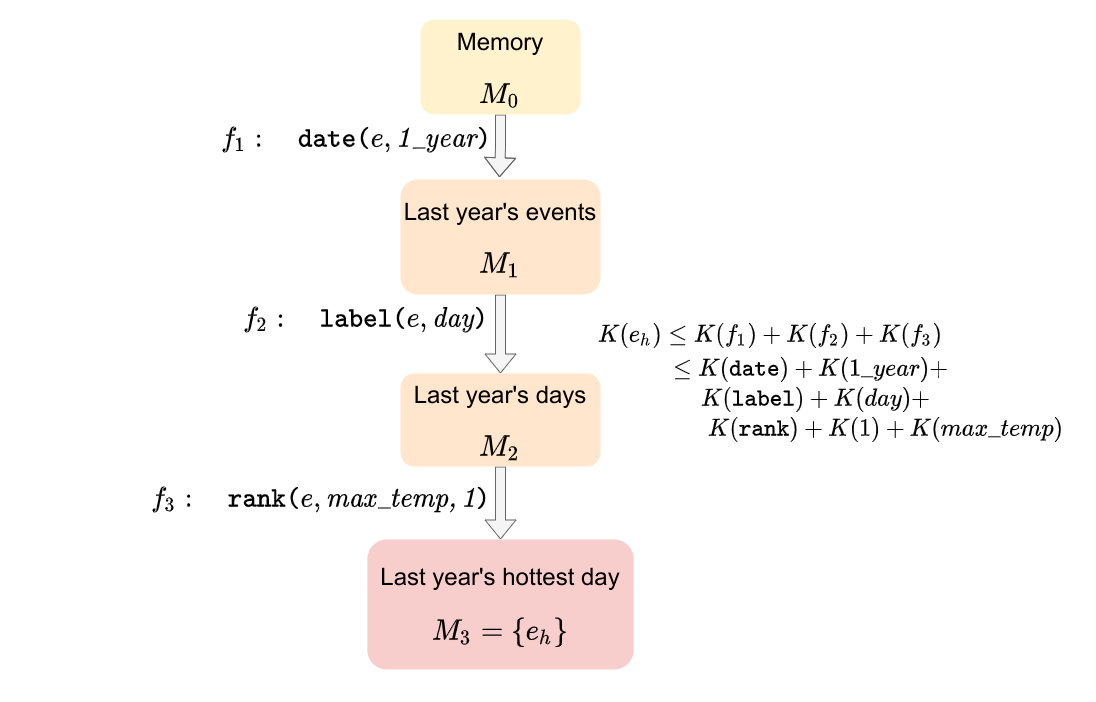
\includegraphics[width=\linewidth]{figures/filters}
  \caption{An example of retrieving an event through successive predicative
    filters. From the base memory (yellow), successive filters select the events
    satisfying their predicates (gray arrows). The operations yields successive
    subsets of the memory (yellow), until a final singleton memory is reach,
    meaning that the successive filters retrieve a unique event from the memory.
    The predicates used for this retrieval path and their arguments,
    $\pi_{1}, \pi_{2}, \pi_{3}, k_{1}, k_{2}, k_{3}$, can be used as a retrieval
    program. Its length gives an upper bound to the description complexity of
    the event $e_{h}$: ``last year's hottest day''.}
  \label{fig:filters}
\end{figure}

To programmatically achieve this computation, we rely on principles from
Algorithmic Information Theory, which provides formal definitions of complexity
and simplicity of objects, which appear to be consistent with human perception
\cite{li_introduction_2008, dessalles2011coincidences, delahaye_numerical_2012}.
 Figure \ref{fig:filters} shows our solution applied to the example description
 ``last year's hottest day''. We assume that
a memory $\mathcal{M}$ is a unordered set of various distinct objects, upon
which can be applied boolean predicates $\pi_{k}$ to describe them. These predicates thus
provide filters $f_{\pi, k}$ that can be applied to the memory, selecting all events
satisfying predicate $\pi_{k}$. By applying successive
filters, we narrow down the size of the memory, until a single event remains.
All the successive filters used to come to this singleton memory constitutes a
\emph{retrieval path}, whose length, in bits, gives an upper bound of the
description complexity of the retrieved event.

The rest of this paper is organized as follows: we first briefly introduce
some notions of Algorithmic Information Theory and its applications in
section~\ref{sec:theory}, then we explicit our methods of computing the
unexpectedness of past events in cyber-physical systems~\ref
{sec:computing}. We illustrate this approach by providing an implementation
relying on a few predicates on events from a smart home simulation~
(section \ref{sec:example}). In section~\ref{sec:related} we briefly review
other related works using complexity theory or trying to explain smart homes
and how our work can be linked with them before exploring potential
extensions of our work in section \ref{sec:future}

\section{Theoretical Background}
\label{sec:theory}
Kolmogorov complexity formally quantifies the amount of information required
for the computation of a finite binary string\footnote{While the definition still
holds for some infinite binary strings (think of the representation of the
decimals of $\pi$), we restrict ourselves to finite strings in this paper.} (or
any object represented by a finite binary
string)\cite{kolmogorov_three_1965,li_introduction_2008}. For such a binary
string $s$, its complexity $K(s)$, is the bit length of the shortest program $p$
which, if given as input to a universal Turing Machine $U$, outputs $s$.
\begin{equation}
  \label{eq:kolmo_def}
  K_{U}(s) = \min_{p}\left\{l(p)|U(p)=s\right\}
\end{equation}

The first notable property of this definition is its universality: while the
choice of the Turing machine $U$ used for the computations appears in the
definition of eq. \ref{eq:kolmo_def}, all results stand, up to an additional
constant. Think, for instance, how any Turing-complete programming language can
be turned into any other language, using a compiler program. In fact, since any
Turing machine $U'$ can be emulated by $U$ from a
finite program $p_{U}$, we have the following inequality:
\begin{equation}
  \label{eq:inequality_univ}
  K_{U}(s) \le l(p_{u}) + K_{U}(s)
\end{equation}

From this first result, we can then define a universal complexity $K(s)$, which
no longer depends on the choice of a Turing machine $U$, such that, for any
machine $U$,
\begin{equation}
  \forall U\in\text{TM}, \forall s, |K(s) - K_{u}(s)| \le C_{U}
\end{equation}
where the additional constant $C_{U}$ does not depend on the object $s$.

It is important to note that the notion of Kolmogorov complexity is not related
to computation complexity, as there is no requirement on the execution time of
the programs, only their length in bits matters for the computation of
complexity. In fact, it can be shown that Kolmogorov complexity is not
computable\cite{li_introduction_2008}. The sketch of the proof is the
following: since the definition of complexity from eq. \ref
{eq:kolm_def} requires to find the shortest of all programs on a given Turing
machine outputting $s$, it requires to run all programs up to a given length
and compare their result to $s$. However, being able to do so means that we
would be able to tell whether these programs terminate. Since the termination
of programs is famously undecidable, by extension, the computation of
Kolmogorov complexity is impossible. One can however easily approximate it with
upper bounds, by exhibiting a program outputting $s$.

Interestingly, Kolmogorov's definition of complexity matches the intuitive
notion and perception of complexity from a human standpoint. For instance, the
complexity of short binary strings evaluated in \cite{delahaye_numerical_2012}
shows similar results to human perception of complex strings and patterns. More
recently, \cite{murena_solving_2020} used Kolmogorov complexity to solve
analogies and showed results close to human expectations.

This bridge between Algorithmic Information Theory and human perception of
complexity is extended to define the notion of simplicity and unexpectedness,
which are considered of uttermost importance in cognitive science\cite
{chater_simplicity_2003}.
\cite{dessalles2011coincidences} proposes a formal definition of the
 unexpectedness $U(e)$ of an event, as the difference between an a-priori
 expected causal complexity $C_{w}(e)$ and the actual observed complexity $C
 (e)$.
\begin{equation}
  \label{eq:unexpected}
  U(e) = |C_{w}(e) - C(e)|
\end{equation}
This result comes from the understanding that, while Kolmogorov complexity is
computed with Turing machine, it can be used as an elegant proxy for modeling
information processing in the human brain, and thus helps design a notion of
simplicity or complexity of events.

Using this measure, it is possible to model phenomenons such as coincidences:
imagine that you happen to run into someone in a park. If this person is not
noticeable, the event will be quite trivial. On the other hand, this person is
your best friend, as the description complexity $C(e)$ drops, the causal
complexity $C_{W}(e)$ remains unchanged, and the event becomes noticeable.

Using these insights from AIT, we propose to measure the complexity of past
events $e$ from a memory $\mathcal{M}$ by considering the quantity
$K(e|\mathcal{M})$, that is the length of the shortest program outputting $e$,
given the entire memory of past events $\mathcal{M}$ as an input. To limit the
search and obtain a computable measure, we limit ourselves to only a subset of
possible programs, which we will now describe.

\section{Computing the unexpectedness of events}
\label{sec:computing}
\subsection{Retrieving an event}
We model the memory as an unordered set $M$ of events $e$. Individual events can
be seen as data points, augmented with a label indicating their nature
(temperature events, failure events, addition/removal events), and a timestamp:
\begin{equation}
  \label{eq:event}
  e = (l, t,\mathcal{D})
\end{equation}
where $l$ is the label, $t$ a timestamp and $\mathcal{D}$ a multi-dimensional
data point representing various characteristics of the events (e.g.~its duration,
the maximum temperature reached, the sensor name, its position).

We define \emph{predicates} as boolean function operating on these events, and
taking an additional argument, encoded as a finite binary string:
\begin{equation}
  \label{eq:predicate}
  \pi : \begin{cases}
    \mathcal{M}\times \{0,1\}^{*} &\mapsto \{0,1\} \\
    (e, k) &\mapsto \pi_{k}(e)
    \end{cases}
\end{equation}
An example of predicate is to use $\pi = \mathtt{year}$ and $k=1$, thus
constructing the predicate $\mathtt{year()}e, Y\mathtt{)}$, which tells whether
the event $e$ occurred $Y$ years ago.

From these predicates, we can construct filter operations on the memory. A
filter operates by selecting the events satisfying a given predicate
$\pi_{k}$ and constructing a resulting memory from these events.
\begin{equation}
  \label{eq:filter}
 f_{\pi, k}(\mathcal{M}) = \left\{e \in \mathcal{M} | \pi_{k}(e) \right\}
\end{equation}
For instance, using the same $\pi = \mathtt{year}$ and $k=1$ as above, we would
build the filter $f_{\pi, k} = \mathtt{last\_{}year}$, which selects all events
that occurred last year.

As the output of a filter applied to the memory $\mathcal{M}$ is another memory
object $\mathcal{M'} = f_{\pi, k}(\mathcal{M})$, we can compose filter
functions. A sequence of such filters, applied in succession, is called a
\emph{retrieval path}
\begin{equation}
\label{eq:ret_def}
p = (f_{\pi_{1}, k_{1}}, \dots, f_{\pi_{n}, k_{n}})
\end{equation}
and by definition
$p(\mathcal{M}) = f_{\pi_{n}, k_{n}}(\dots(f_{\pi_{1}, k_{1}}(\mathcal{M})))$.
In case the result of the operation $p(\mathcal{M})$ contains a single element
$e$, we say that the path $p$ \emph{retrieves} the element $e$ from $\mathcal{M}$, and write
$p(\mathcal{M}) = e$.

\subsection{Description complexity of events}

% From the previous definitions, we then estimate the complexity of events as the
% ``simplest'' way of retrieving them from the memory, by applying successive
% filters. A retrieval path composed of various filters
% $p = f_{1} = f_{\pi_{1}, k_{1}}, f_{2} = f_{\pi_{2}, k_{2}}, \dots, f_{n} = f_{\pi_{n}, k_{n}}$
% is said to \emph{retrieve} an event $e$ from a memory $\mathcal{M}$ if and only
% if
% $p(\mathcal{M}) = f_{1} \circ f_{2} \circ \dots \circ f_{n} (\mathcal{M}) = \{e\}$.
% For an event $e$, if such a path exist, its complexity can be bounded by
% $K(p) = \sum_{f_{\pi, k} \in p} l(\pi) + l(k)$, the complexity of the retrieval
% path being the sum of the bit lengths required to describe the predicates $\pi$
% and their arguments $k$.

As presented in sec. \ref{sec:theory}, we are interested in computing the
Kolmogorov complexity of an event $e$, conditionned on the memory $\mathcal{M}$.
As this quantity is not computable, we use the previous definitions of retrieval
paths and approximate the quantity $K(e|\mathcal{M})$ by the lenght of the
shortest retrieval path $p$ retrieving $e$ from $\mathcal{M}$.

Given that all predicate concepts can be described by a prefix program of length
$l(\pi)$, and their arguments in length $l(k)$, each retrieval path $p$ can be
described by the sequence of prefix description of all the predicate concepts and
arguments used to construct its filters:

\begin{equation}
K(p) = l((f_{\pi_{1}, k_{1}}, \dots, f_{\pi{n}, k_{n}})) = \sum_{i=0}^{n} l(\pi_{i}) + l(k_{i})
\end{equation}

Using this definition of the lenght of a retrieval path, we can compute the
estimation for the complexity $K(e|\mathcal{M})$, which, for clarity, we will
denote simply by $K(e)$ for the rest of this paper.

\begin{equation}
  \label{eq:desc_k}
  K(e) \approx \min_{p | p(\mathcal{M}) = e} K(p) = \min_{p | p(\mathcal{M})=e} \sum_{f_{\pi, k} \in p} l(\pi) + l(k)
\end{equation}

\begin{algorithm}
  $\mathtt{current_{explore}} \leftarrow [(\mathcal{M}, 0)]$ \;
  $\mathtt{future_{explore} \leftarrow} [\;]$ \;
  $\mathtt{pass} \leftarrow 0$ \;
  $\mathtt{K(e)} \leftarrow +\infty$ \;
  \While{$\mathtt{current_{explore}} \neq [\;]$ \textbf{and} $\mathtt{pass} < \mathtt{max\_pass}$}{
    \For{$(\mathtt{M_{prev}}, \mathtt{K_{prev}}) \in \mathtt{current_{explore}}$}{
      \For{$\mathtt{\pi \in \mathcal{P}}$}{
        \For{$\mathtt{k \in \{0,1\}^{*}}$}{
          $\mathtt{K_{current} \leftarrow l(\pi) + l(k) + K_{prev}}$ \;
          \If{$\mathtt{K_{current}} > \mathtt{max_{complex}}$}{
            \textbf{break} \;
          }
          $\mathtt{M'} \leftarrow f_{\pi,k}(\mathtt{M_{prev}})$ \;
          \eIf{$\mathtt{M'} = \mathtt{\{e\}}$}{
            $\mathtt{K(e) \leftarrow \min(K(e), K_{current})}$ \;
          }{
            $\mathtt{future_{explore}.append((M', K_{current}))}$\;
          }
        }
      }
    }
    $\mathtt{current_{explore}} \leftarrow \mathtt{future_{explore}}$ \;
    $\mathtt{future_{explore}} \leftarrow [\;]$ \;
    $\texttt{pass} \leftarrow \mathtt{pass} + 1$\;
  }
  \caption{Iterative computation of the approximate complexity}
  \label{alg:complex_iter}
\end{algorithm}

The definition used for description complexity in eq. \ref{eq:desc_k} allows for
a direct implementation, which is shown in alg. \ref{alg:complex_iter}. This
algorithm operates iteratively: starting with the base memory $\mathcal{M}$
(line 1), we apply all possible predicate concepts $\pi$ from a given set
$\mathcal{P}$ and programs $k$ (lines 6-7), up to a given length $\mathtt
{max\_len}$ bits, and apply them: $M' = f_{\pi, k}(M)$ (line 12). We then store
the pairs $(M', \mathtt{len(}\pi, k\mathtt{)})$ in an array $\mathtt{future_
{explore}}$. At the end of the iteration, the results of the filters become the
memories which will be explored during the next iteration(lines 21--23). Each
pass thus explore retrieval paths of increasing length. When a singleton memory
is reached, the complexity of its unique element is upper-bounded with the
length of the corresponding retrieval path (line 14).

\subsection{Computing an unexpectedness measure}
Equation \ref{eq:unexpected} gives a universal definition of unexpectedness, as
the difference between the complexity of the phenomenon generating an event and
the complexity required to describe this event. In our particular application
case, we may directly use the description complexity $K(e)$ as defined in
\ref{eq:desc_k}.

The term $C_{w}(e)$ from eq. \ref{eq:unexpected} is harder to formally
fit into our canvas. As $C_{w}$ is defined as the shortest program a
``W-machine'' replicating the world's behavior, based on the person's
knowledge\cite{dessalles2011coincidences}, it is convenient to understand this
term as the expectation one would have regarding the complexity of the event
$e$, \emph{before} actually evaluating it.

A possible proxy for this quantity is to compute the average complexity
of \emph{similar} events. Still, difficulty remains in the definition of what
can be considered \emph{similar} events. Given that we have already used the
notion of predicates to describe the events and compute their description
complexity, we can use them as simple metrics for similarity: for each predicate
$\pi$ satisfied by $e$, we can define a set of similar events $N_{\pi}(e)$ as
all the events also satisfying $\pi$.

\begin{equation}
\label{eq:similar}
N_{\pi}(e) = \{e'\in \mathcal{M}, \pi(e') \wedge e' \neq e\}
\end{equation}

Now, when considering, for all possible predicates $\pi$, the corresponding
neighborhoods $N_{\pi}(e)$, with the convention that $N_{\pi}(e) = \emptyset$
if $\pi(e) = \bot$, we can compute an average expected complexity for $e$:

\begin{equation}
\label{eq:expected}
K_{exp}(e) = \frac{
                    \sum_{\pi} \sum_{e' \in N_{\pi}(e)} K(e')
                  }{
                    \sum_{\pi} |N_{\pi}(e)|
                  }
\end{equation}

The definition used for the expected complexity of the event $e$ in eq.
\ref{eq:expected} holds the intuition of favoring more similar events: if $e'$
is \emph{very} similar to $e$, it will appear in many neighborhoods, since it
satisfies mostly the same predicates as $e$. Therefore, its complexity term will
be present in more terms in eq. \ref{eq:expected}, and will weight more towards
the final result.

\subsection{From memorability to abduction}
% On peut étendre la définition utilisée pour la surprise en faisant intervenir
% les prédicats'' `sympathiques` par rapport à ce que l'on questionne.
The problem of the abductive inference is different from the basic computation
of the memorability score. Here, \emph{knowing} that we want to find a cause $c$
to an observed effect $e$, we try to find the most remarkable event in past
memory in that regards. While our ``memorability'' score aims to identify the
most remarkable events, it does not take into account the added knowledge about
the effect $e$ that is available for abductive inference.

This added knowledge would however influence the unexpectedness of a possible
cause $c$, from eq. \ref{eq:unexpected}: even though the causal complexity
$C_{W}(c)$ is likely to remain unchanged, as it relies on the model of the world in
the person's mind, the description complexity $C(c)$ is replaced with the
conditional complexity $C(c|e)$, as the knowledge of $e$ is included in the
problem's data.

In our canvas of predicative filtering, this corresponds to adding for free, in
terms of program length, information about $e$ to predicates. This translates
into considering relative order between events: when investigating a cause for
an anomaly in the living-rooms, other anomalies occurring in the same
living-room will be simpler, since the location ``living-room'' is already known
from knowing the consequence. In terms of predicates, we therefore append a
description of $e$ to all programs $k$ of predicates:
$\pi_{k}(c) = \pi_{k::e}(c)$, where $::$ is the append operation.

This leads to another score $Abd(c,e)$ (abduction score of effect $c$ for cause
$e$), which is defined similarly to the description complexity in eq.
\ref{eq:desc_k} and using relative filters.

\begin{equation}
  \label{eq:abd_k}
  Abd(c) = \min_{p | p(\mathcal{M}|e) = c} K(p) = \min_{p | p(\mathcal{M}|e)=c} \sum_{f_{\pi, k} \in p} l(\pi) + l(k)
\end{equation}
This abduction score translates the additional information provided to the
system when answering a user's request. As such, it encapsulates the idea
presented as the motivation of this paper: when confronted to a surprising
situation, and with no other source of information, it can be used as a metrics
to find relevant possible surprising causes to the observed consequence.

\section{Implementation Example}
\label{sec:example}
\subsection{Setup}
To test our approach, we set up an experimental smart home setup. This choice of
configuration is motivated by the challenges posed by smart homes for abductive
inference: i) as the number of connected devices increases, more events are
recorded, making the detection of memorable events more important; ii) smart
homes are prone to undergo atypical situations, highly dependent on the context,
for which pre-established relations might fail to find good abduction
candidates. Furthermore, the choice was also motivated by the ease of application: as
previous works exist on smart homes, it is possible to simulate their behavior
and quickly generate data to extract events from and test our methods.


% In order to provide an acceptable setup to our experiments, we used the scenario
% of smart homes. This kind of scenario is a prime example of situations where
% innovative methods of abduction can prove useful, for various reasons: i) as the
% number of sensors grows with the number of equipped devices in the house, not
% all recorded events are useful and should be remembered over long period of
% time; ii) atypical situations, which are the ones where abduction is most likely
% to be used (to explain situations to the user, or to solve a conflict), are also
% where the lack of past data makes knowledge acquisition hard.

To carry out the simulation, we built custom modules into the existing iCasa
smart home simulator\cite{lalanda_self-aware_2017}. This simulation platform
allows for simulating autonomic systems, handling internal communications,
injection of new components at runtime, deletion or change of existing
components. As such, we used a basic scenario consisting of a house of 4 rooms,
a single user, and an outdoor zone. All four rooms of the house are equipped
with a temperature controller system, monitoring and controlling heaters (fig.
\ref{fig:view}).

\begin{figure}[ht]
  \centering
  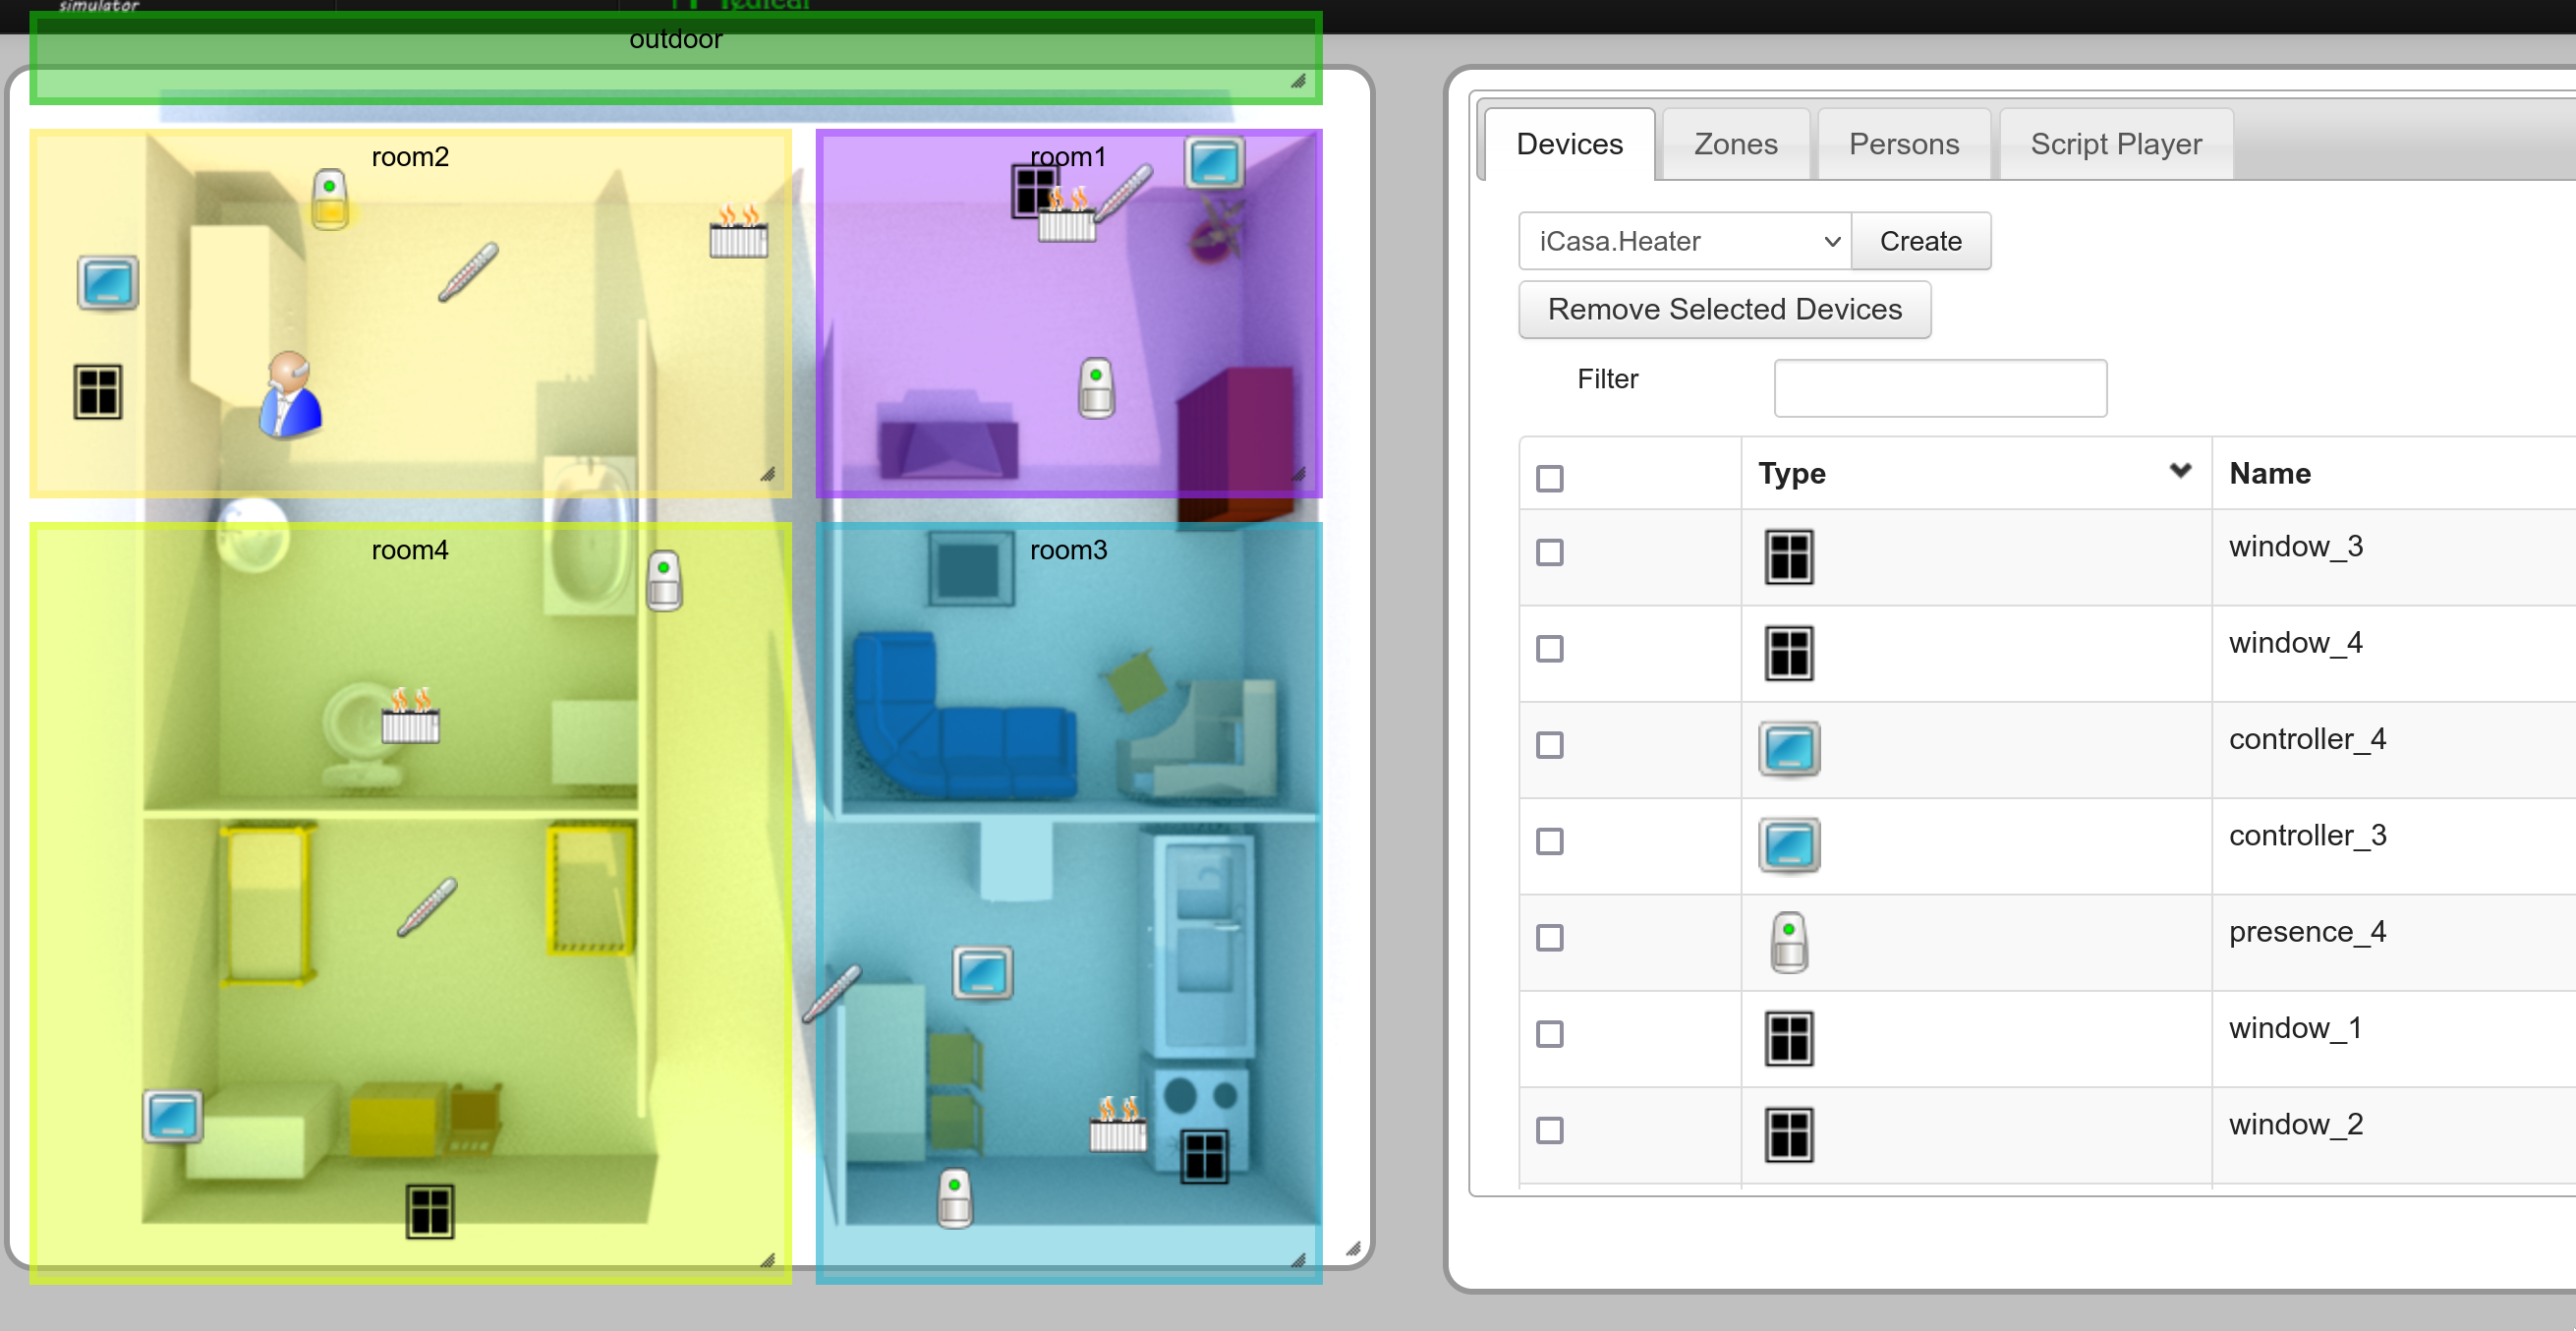
\includegraphics[width=\linewidth]{figures/simulator}
  \caption{View of the simulator's web interface provided by iCasa. The four
    rooms are visible, with their equipment and the user.}
  \label{fig:view}
\end{figure}

Using this basis, we implemented a scenario spanning over 420 days, and
comprising a daily cycle of outdoor weather (temperature and sunlight), as well
as user's movements. All these daily changes create non-noticeable events,
serving as a background noise for our experiments. To produce outstanding
events, we randomly generated around twenty events, spanning over the whole
duration of the simulation, of different kinds:

\begin{itemize}
    \item Unusual weather: the outdoor conditions are set to unusually high or
        low temperatures.
    \item Heater failures: heater can fail, making them turning off regardless
        of the command they receive.
    \item User's vacation: the user go out of the building for an extended
        period of time.
    \item Device removal/addition: a device is removed, or another one is added
        to the system.
\end{itemize}


\begin{figure}[ht]
  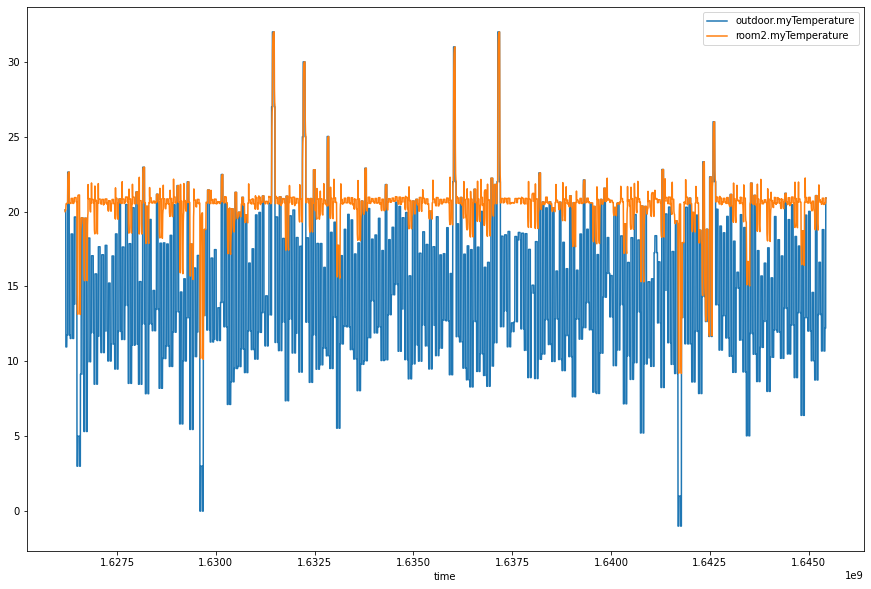
\includegraphics[width=\linewidth]{figures/ts_example}
  \caption{Time series data from the simulation: outdoor temperature (blue) and
    controller temperature of a room (blue). On different occasion, the
    controlled temperature deviates from its setting (21°C). We will evaluate if
  our system finds these deviations as memorable, and if it can propose causal
  hypotheses.}
  \label{fig:ts_example}
\end{figure}

The values of all devices and zones variables was regularly monitored throughout
the simulation run, and the resulting data, which an excerpt is shown in figure
\ref{fig:ts_example} can later be used as a basis for our experiments.


\subsection{Implementing the complexity computation}

For the implementation of our method, we first needed to identify and
characterize events from the time series data generated by the iCasa simulation.
Since this is not the focus point of our present work (see sec.
\ref{sec:related}), we simply apply threshold and pre-computed conditions based
detection to create a base of events.

This base of events consists the basis of the initial memory $\mathcal{M}$ used
for computations.
We then implemented a small number of predicate concepts:
\begin{itemize}
        \item \texttt{label(e, k)}: whether the event $e$ has the label ranked
        $k^{th}$ in the memory.
        \item \texttt{rank(e, k)}: whether the event $e$ has the rank $k_{1}$
        along axis $k_{2}$, where $k$ is a unique encoding for $(k_{1}, k_{2})$.
        \item \texttt{day(e, k)}: whether the event $e$ occurred $k$ days ago.
        \item \texttt{month(e, k)}: whether the event $e$ occurred $k$ months
        ago.
        \item \texttt{location(e, k)}: whether the event $e$ occurred in zone
        $k$.
\end{itemize}

With a straightforward implementation of memory, predicates and filters, the
implementation of alg. \ref{alg:complex_iter} worked, but, as expected, took too
long to be usable in realistic scenarios with hundreds or thousands of events to
consider. In order to facilitate and speed up computations, we also implemented
the following improvements:
\begin{itemize}
  \item The memory object was augmented with various built-in rankings, allowing
  for faster operations during future filtering. For instance, since the memory
  object keeps a mapping from timestamps to events, which allows to quickly
  filter by date without having to loop over each stored element. This mapping,
  however, is not directly used to retrieve an event from the outside, as to
  preserve the theoretical model of memory as an unordered set presented in
  section \ref{sec:computing}.

  \item Each of these predicates holds the property that, in addition to
  \texttt{True} and \texttt{False}, they can return another value,
  \texttt{None}, which is theoretically treated as \texttt{False} but carries
  the additional information that this predicate concept will also be false for
  any other element of the memory for any subsequent program $k$. This allows to
  effectively break the innermost loop in alg. \ref{alg:complex_iter}.

  \item Some of the filters, for instance date or rank filters, were
  hard-written to select from the pre-computed mappings of the memory objects
  rather than testing a predicate over all memory elements.
\end{itemize}


\subsection{Results}

\subsubsection{Memorability}

The results of the description complexity evaluation, for the described setup,
are shown in fig. \ref{fig:computed_cplx}. The entire computation, over 4
iterations (meaning that retrieval paths contained at most 4 filters), took
around 30 seconds on a modern commercial laptop with an i7-8700u CPU.

A main sequence of ``usual'' events, which complexity is roughly a logarithm of
the elapsed time since their occurrence, is visible. This corresponds to events
for which the best retrieval path consists of a time description (e.g. ``2
months and 12 days ago''). On the other hand, some events stand out in terms of
complexity: some appear simpler, as they can be distinguished by using their
rank alongside an axis (``the hottest day'', ``the second longest user's
absence''), or the rare occurrence of their kind (``the only fault on the heater'').

\begin{figure}[ht]
  \centering
  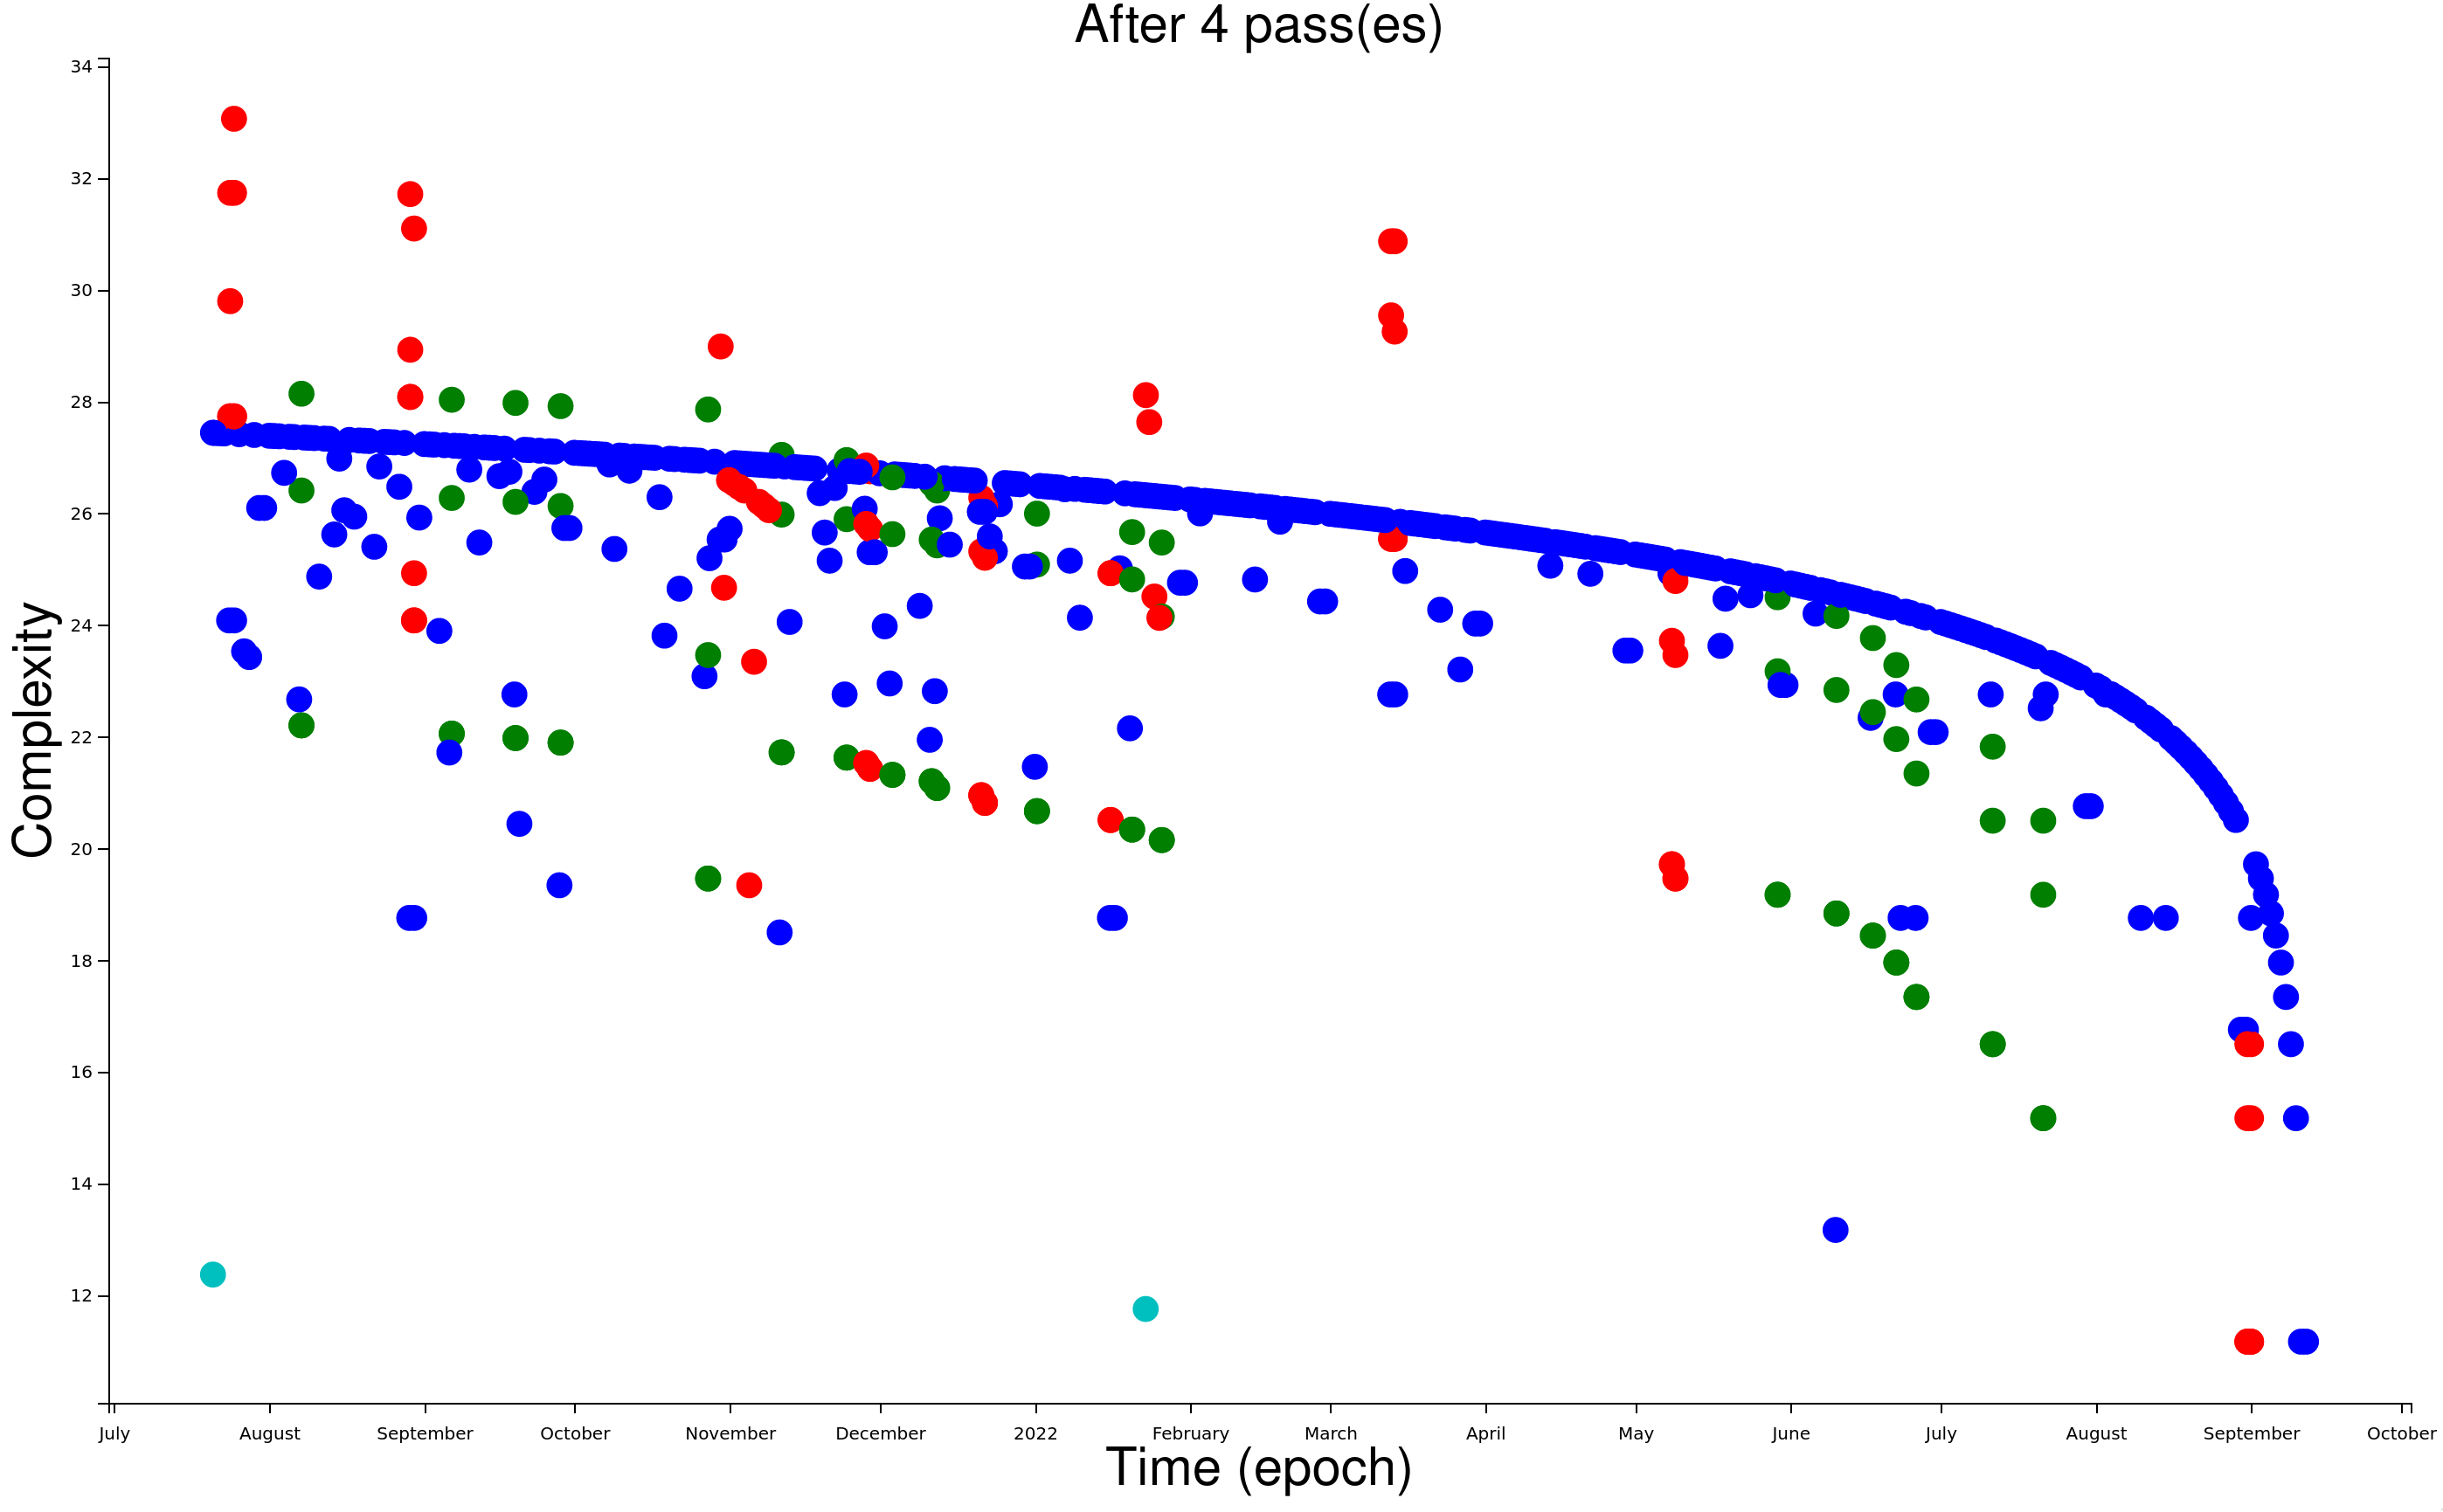
\includegraphics[width=\linewidth]{figures/complexities_computed}
  \caption{The computed complexities of events with at most retrieval paths of
    length at most 4. Events of type ``day'' (blue), ``hot'' (green), ``cold''
    (red), ``device removal''(cyan) are shown.}
  \label{fig:computed_cplx}
\end{figure}

Computing the ``memorability score'', which is shown in fig. \ref{fig:result1},
highlights these aforementioned events from the main ``usual'' sequence. Since
the computation of this measure treats unusually complex or simple events the
same way (from the absolute value operation in eq. \ref{eq:unexpected}), we
observe that some events are memorable due to their context only. For instance,
a temperature anomaly occurring simultaneously to many other anomalies is
notable, as it is costlier than expected to distinguish it from its neighbors.

\begin{figure}[ht]
  \centering
  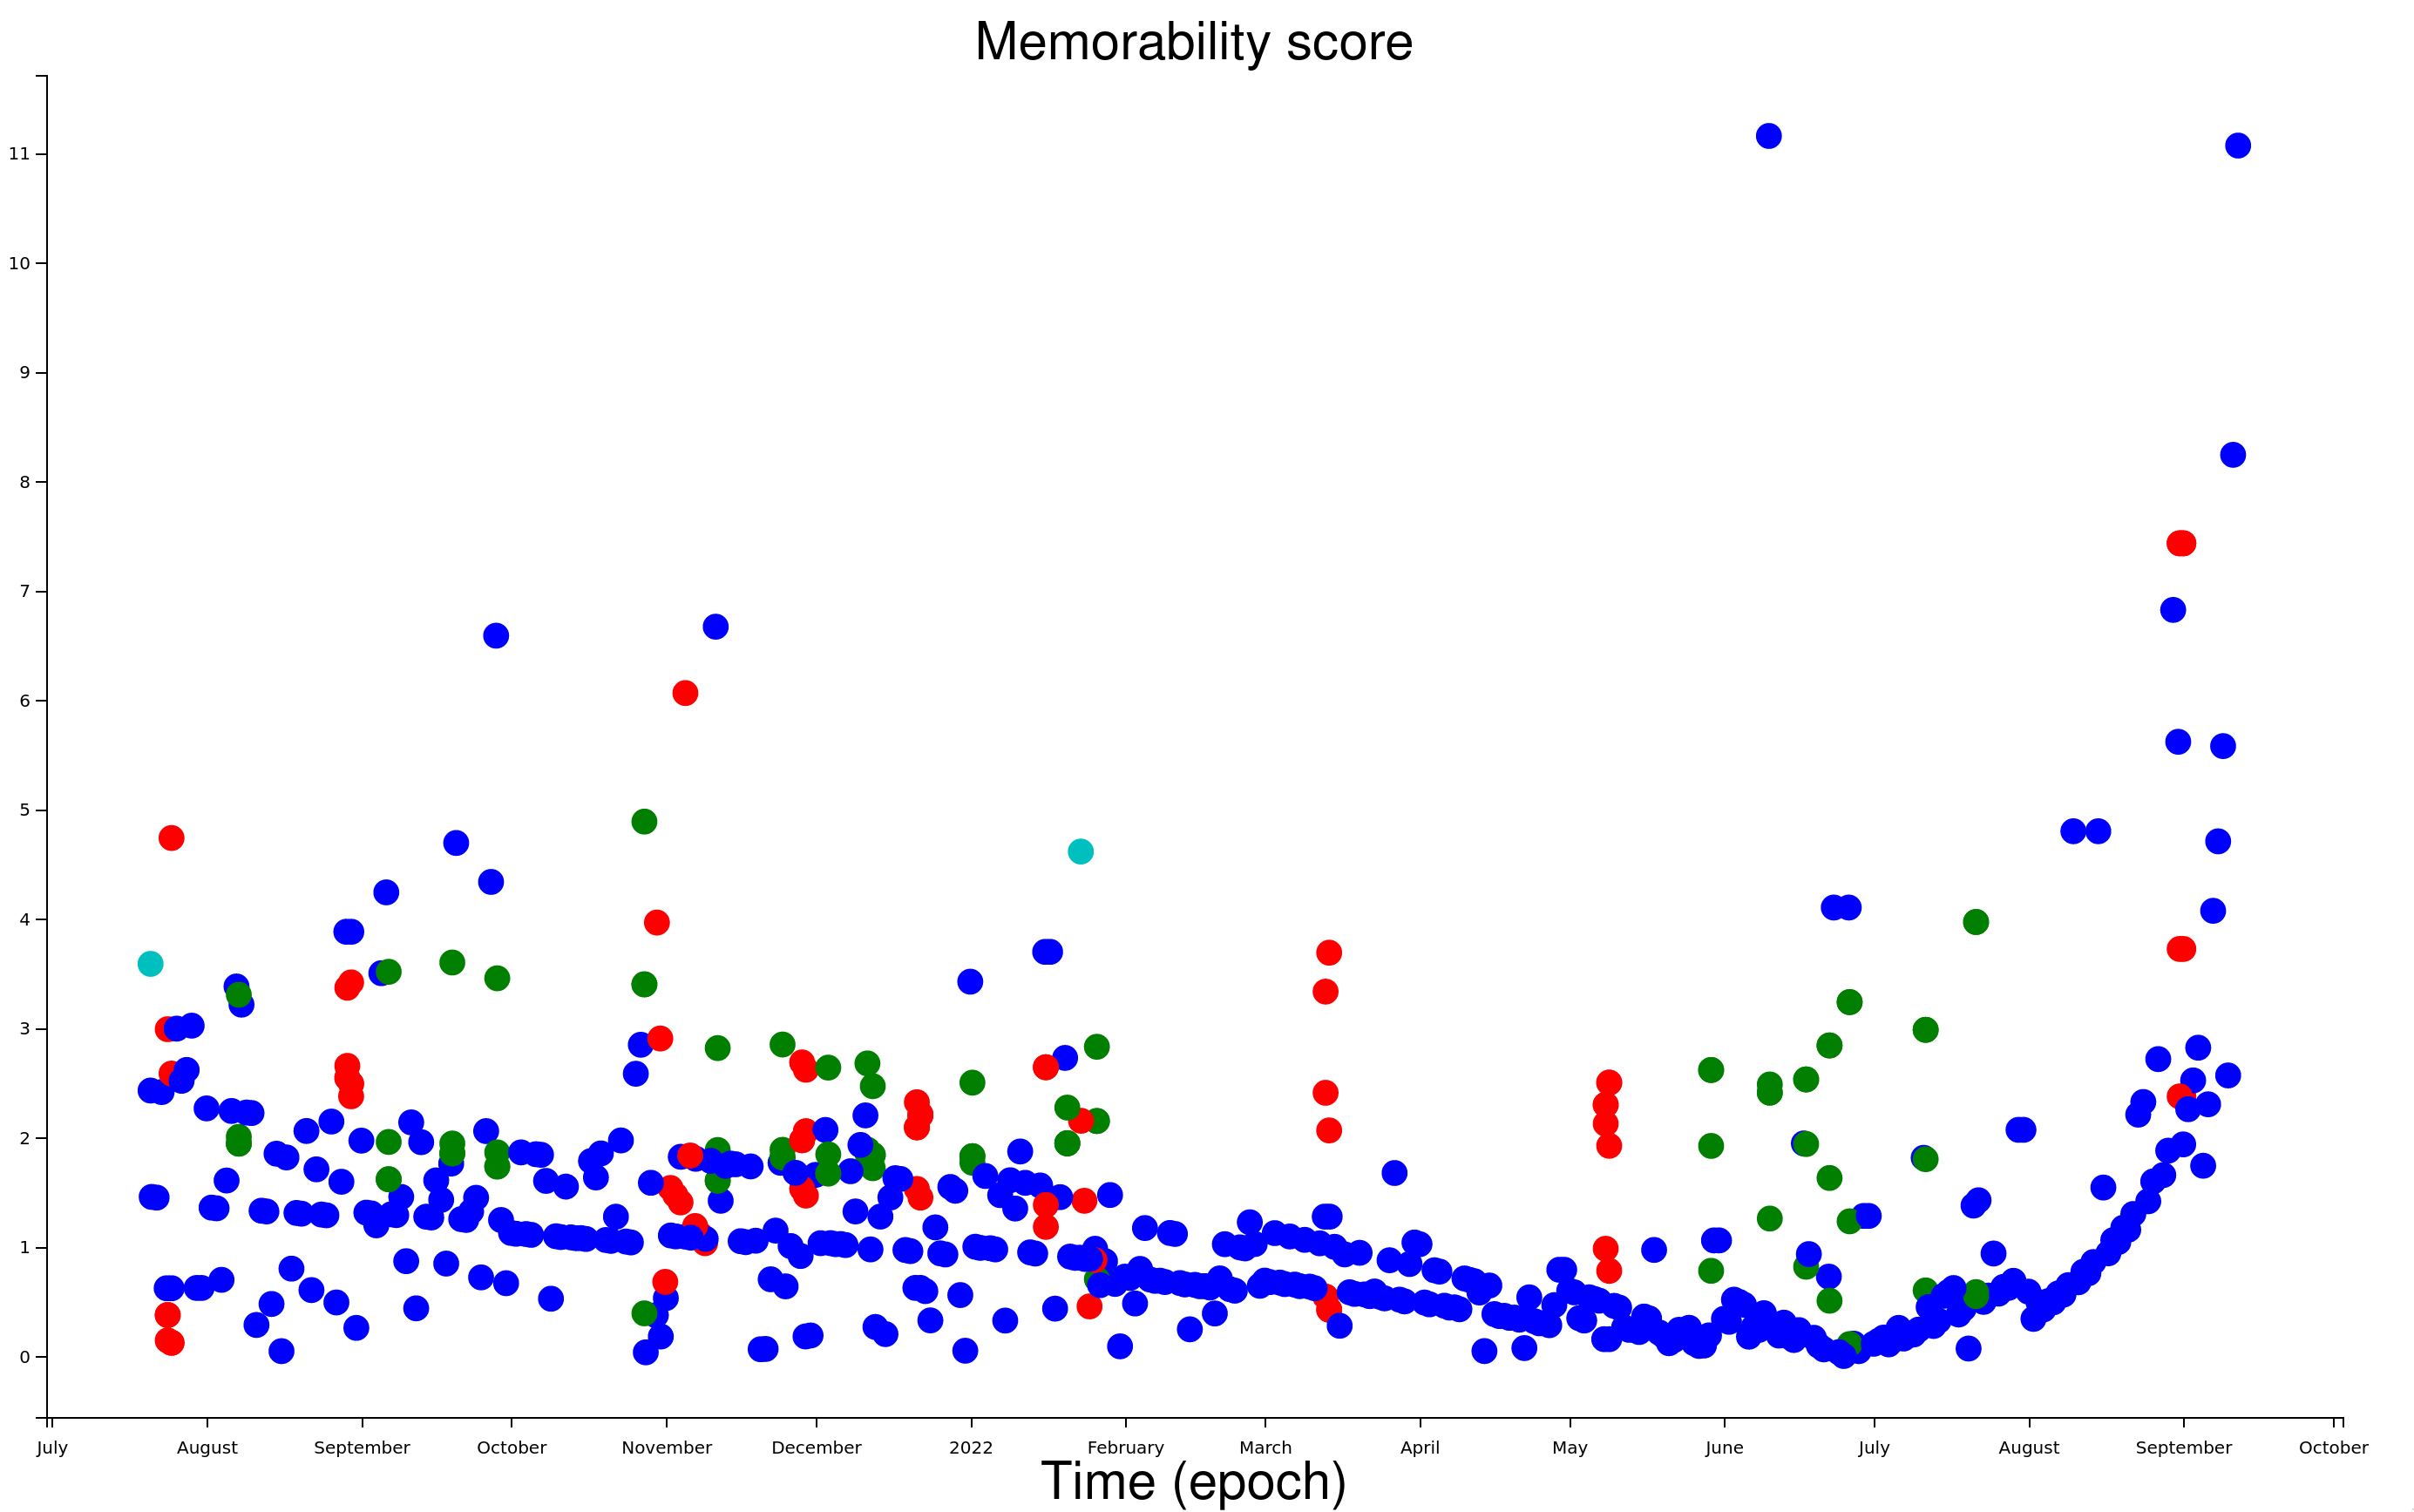
\includegraphics[width=\linewidth]{figures/complexities_surprises}
  \caption{Memorability score for events in the memory}
  \label{fig:result1}
\end{figure}

Given that we generated the data used for this experiment, it is possible to
flag all perturbation events from the usual daily events and evaluate how a
detection based on ``memorability'' score would succeed in distinguishing these
events. The result is presented as a ROC curve in fig. \ref{fig:roc}.

\begin{figure}[ht]
  \centering
  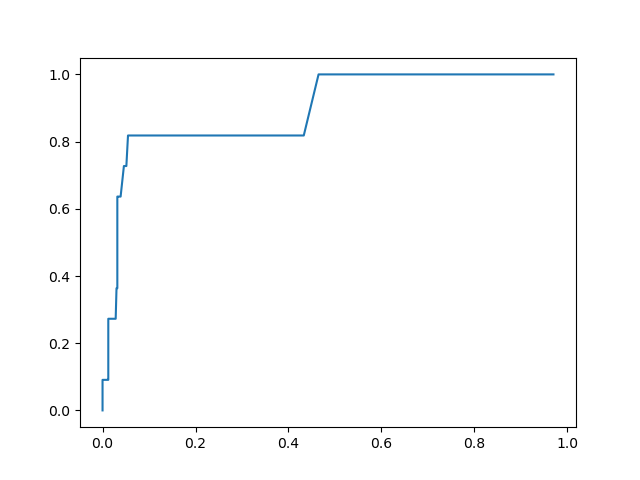
\includegraphics[width=\linewidth]{./figures/roc}
  \caption{Experimental ROC curve (True Positive Rate against False Positive
   Rate) for a classifier based on our memorability score. Measures consider 23
   manually flagged events as memorable (events added to the background noise
   as described in Section~\ref{sec:example}.)}
  \label{fig:roc}
\end{figure}
\subsubsection{Abduction}

As an illustration of the abductive inference possible by using the memorability
score, we used as a target consequence the temperature drop visible in the raw
time series data from our scenario (fig \ref{fig:ts_example}).

% TODO
\textbf{TODO}

\section{Related Works}
\label{sec:related}
Our work is intended to be integrated into larger-scale frameworks to monitor 
and detect events in complex environment such as smart homes. In these works, the
approach to smart homes is often regarded as self-organizing systems \cite{kramer_rigorous_2009,kounev_notion_2017}. As such, they present capacities of adaptation to new goals, 
new components, new environment. A commonly used approach is the principle of 
autonomic system, which minimizes user's intervention for management of the 
system \cite{kounev_notion_2017,kephart_vision_2003}.

We want to inscribe our work among other classical concurrent approaches to 
abduction. In situations where more data is available, we could for instance rely
on correlation or causal inference from known relations \cite{peters_elements_2017,fadiga_or_2021}.
Previous relations between inference and complexity have been studied. In fact, the 
case of inference was one of the motivations for R. Solomonoff to introduce his 
universal algorithmic probability \cite{solomonoff_formal_1964} as a tool to 
reach an idealized inference machine, creating the notion of complexity concomitantly 
to Kolmogorov. Subsequently, notions of complexity re-emerged in causal inference: 
\cite{janzing_causal_2010} found, when a causal link exists between two random variables,
considering the direct joint probability is simpler, in terms of Kolmogorov complexity, 
than the inverse direction.

The topic of finding events from streams of time series data has already been explored in many ways. 
\cite{aggarwal_outlier_2017} provides good review of modern approaches and techniques
in the field.

While all these works advocate in favor of a strong link between complexity and the 
discovery of causes, not other works extends the notion up to the point we propose in this
work, using complexity only as a tool for inference. 

\section{Perspectives}
\label{sec:future}
The main purpose of the present paper is to show the possible connections
between existing definitions of simplicity from cognitive science, Algorithmic
Information Theory and a practical use case in cyber-physical systems. As such,
many further improvements can be done to pave the way towards a better
integration and performance for anomaly detection or abduction.

First, the main limitation of the current approach is the requirement of
predefined predicate concepts, from which the different filters are constructed.
As an extension, we suggest that in the future, we could explore online
generation of such predicate. A possibility would be to analyze discriminating
dimensions of incoming data and create predicate as to name these differences,
similar to the contrast operations proposed in \cite{dessalles_conceptual_2015,
  gardenfors2004conceptual}. For instance, the predicate concept $\mathtt{hot}$
can be discovered by discriminating a recent hot day along the
temperature axis and naming the difference with the prototypical day.

While the execution time is not part of the theoretical view of complexity, it
is of prime importance for practical applications, especially when one considers
implementation into real-time systems or embedded devices. While the computation
we propose appear to be heavy, and possibly heavier as the number of allowed
predicates grows, significant time savings can be achieve by trimming the base
memory of past events deemed the most ``non memorable''. For instance, one can
only retains the 100 most memorable events from the past. The difficulty with
this approach is that such operations should be done in a manner to not
interfere with the complexity computations for new elements: by forgetting some
past events, even uninteresting ones, one should make sure to keep track of what
made the interesting ones, interesting. Investigation of how to do so can pave
the way towards practical implementations and dynamic selection of interesting
events and help reducing the memory and computation cost of data-driven applications.


\section{Conclusion}


\bibliographystyle{IEEEtran}
\bibliography{biblio.bib}

\end{document}
